\documentclass[11pt,a4paper]{article}

\usepackage[utf8]{inputenc}
\usepackage[spanish,mexico]{babel}

\usepackage{amsmath, amssymb, amsthm}
\usepackage{mathrsfs}
\usepackage{appendix}
\usepackage{minted}	

%pdflatex -synctex=1 -interaction=nonstopmode --shell-escape %.tex


\usepackage{hyperref}
\usepackage{captdef}

\usepackage{psfrag}
\usepackage{graphicx}
%\usepackage{subfig}
\usepackage{color}
\usepackage{multicol} 

%\usepackage{fancyhdr}
%\pagestyle{fancy}
%\fancyhf{}


\usepackage{cancel}
\usepackage[usenames,dvipsnames,svgnames,table]{xcolor}
\usepackage[left=2cm,right=2cm,top=2cm,bottom=2cm]{geometry}
\usepackage{caption}
\usepackage{subcaption}
%\renewcommand{\baselinestretch}{1.5}

\usepackage{hyperref}
%\usepackage[hidelinks]{hyperref} 
\hypersetup{
    colorlinks=true,
    linkcolor=blue,
    filecolor=magenta,      
    urlcolor=cyan,
    }

\begin{document}
\thispagestyle{empty}

\includegraphics[height=3.5cm]{escudoCiencias.pdf}
\vspace{-3.8cm}
\begin{flushright}
\hspace{4cm}
{\Large\textbf{Sobre los sistemas lineales y los no lineales}\\
Proyecto de Tesis}
\vspace{0.3cm}\\
\begin{large}Autor: Rodrigo Vega Vilchis.\end{large}\\
\begin{footnotesize}
Correo: rockdrigo6@ciencias.unam.mx\\
\hspace{2.05cm}{\color{white}.}\\
\end{footnotesize}
\vspace{0.1cm}
\begin{large}
Fecha: 26 Febrero, 2024\end{large}\\
\end{flushright}
%\vspace{.4cm}
 \hrule height1pt\vspace{.5cm}
\begin{abstract}
Este primer pasaje ha servido para retomar las ideas principales de los sistemas lineales y no lineales para poder ir desarrollando en una base sólida en sistemas no lineales de $N$ especies. Existen 3 tipos de estabilidad dadas por fuentes, sumideros y puntos sillas; la estabilidad depende directamente del signo de la parte real de los eigenvalores del sistema: si todos los eigenvalores tienen parte real negativa se dice que el sistema es estable. Las interacciones presentes en el sistema pueden dar lugar a sistemas estables o inestables, los términos negativos de la matriz de interacciones $A$ representa cooperación entre especies y propicia la coexistencia de las especies.
\end{abstract}

\section{Introducción}

Una de las razones por las que he decidido hacer una serie de pasajes es para tener documentado el progreso que he llevado hasta ahora. Tengo muchas entradas en blocs de notas o en notion pero no esta en un formato profesional del cual pueda disponer de una lectura cómoda y organizada. También el ejercicio de esta actividad será el de retomar la escritura e ir desenpolvando las habilidades de expresión escrita; al mismo tiempo irlas mejorando para llegar bien curtidos al -producto final que será el trabajo de tesis. Desenpolvar las habilidades de Latex también será oportuno.\\
\\
Comenzaré el pasaje con una reflexión personal de las ecuaciones diferenciales, de acuerdo a lo que conozco y la experiencia que tengo al respecto. Las definiría como las herramientas fundamentales para poder medir, cuantificar, predecir, modelar el cambio o el movimiento de las cosas en el universo. Podemos ser pedagógicos y jugar con las derivadas de tal forma que se establezca la trayectoria de un proyectil, o la dinámica del famosísimo oscilador armónico. Estos ejercicios suelen ser importantes para la parte formativa, saber resolver las matemáticas y entender el trasfondo de lo que representa la solución de las ecuaciones es sublime.\\
\\
Sin embargo, es posible subir el nivel de complejidad al tipo de cambio o dinámica que se quieran estudiar, con las variables e hipótesis adecuadas se puede generar un modelo que nos ayude a comprender un pedazo de la naturaleza. El ejemplo clásico que nos adentra hacia la temática de la tesis es sobre la dinámica de poblaciones. Es posible definir la siguiente ecuación
$$\frac{dP}{dt}=kP$$
Donde $P(t)$ corresponde a una población en un determinado instante de tiempo $t$, la ecuación nos indica que la razón de cambio de la población con respecto del tiempo es proporcional a la misma población, es decir, que conforme pasa el tiempo, la población irá creciendo $kP$ veces. Resolviendo la ecuación tenemos 
$$P(t)=P_0e^{kt}$$
La población crecerá de manera exponencial desde cierta población inicial ($P_0$), sin embargo la función exponencial es creciente al infinito conforme $t\to\infty$ y debido a temas de recursos y ambientes, se sabe que es imposible que una población pueda presentar dicho comportamiento. Quizás para tiempos cortos sea posible adaptar este modelo a la realidad, pero es necesario anexar más hipótesis para mejorarlo y asemejarlo más a la realidad. Una de las propuestas para mejorar el modelo es volverlo logístico de la siguiente manera
\begin{equation}\label{eq:logistica}
\frac{dP}{dt}=rP\left(1-\frac{P}{K}\right)
\end{equation}
Por un lado la ecuación sigue teniendo un crecimiento exponencial pero sucede que cuando la población se va acercando a una capacidad de carga del sistema $K$ (que viene dado por las limitantes del sistema), el crecimiento va decreciendo hasta que se estabiliza en dicho límite.
\begin{figure}[t!]
        \centering
        \begin{subfigure}[h]{0.5\textwidth} 
            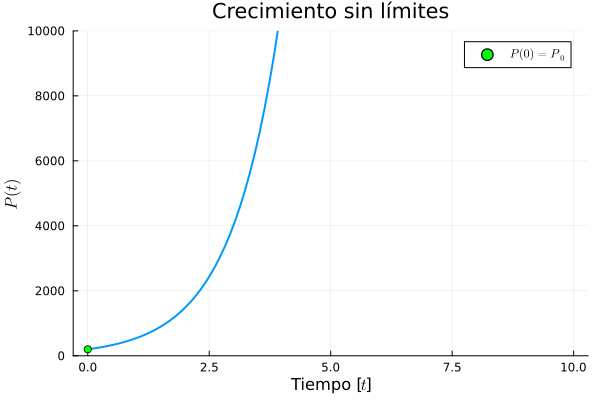
\includegraphics[width=\textwidth]{Crecimiento sin limites}
            \caption{Modelo de población sin resitricciones y con crecimiento al infinito}
            \label{fig:sinLim}
        \end{subfigure} 
        \hfill 
        \begin{subfigure}[h]{0.49\textwidth} 
            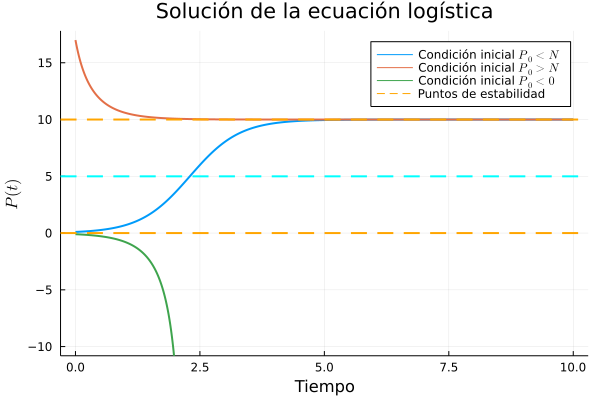
\includegraphics[width=\textwidth]{Ecuación logística}
            \caption{Modelo de población con capacidad de carga dada por limitaciones en el ambiente.}
            \label{fig:logistico}
        \end{subfigure}
\end{figure}

\section{Sistemas lineales}

La ecuación logística será nuestra piedra angular en esta aventura de investigación (de la que ya llevo un gran rato, quizás dos años), no sin antes resaltar que se trata de una ecuación no lineal. La diferencia entre las ecuaciones lineales y las no lineales recae en el hecho de que las primeras responden al principio de superposicición, es decir, puedes sumar las soluciones posibles del sistema y seguirá siendo solución. Los sistemas no lineales no poseen dicha ventaja y mayormente son más complicados de resolver debido a que no suelen tener solución analítica.\\
\\
Puede que la simple ecuación logística (\ref{eq:logistica}) tenga su respectiva solución analítica pero cuando queremos generar la interacción de varias poblaciones, la tarea en verdad se vuelve complicada de atender. Para poder estudiar el comportamiento de varias poblaciones que interactúan entre sí es necesario primero pasar por el contexto de los sistemas lineales y el tipo de dinámica que producen; por el tipo de dinámica que producen me refiero a las fuentes y atractores del sistema. Un sistema lineal no es más que un conjunto de ecuaciones diferenciales de primer grado que interaccionan entre sí. Cualquier cantidad que intervenga en el sistema necesariamente interacciona con las otras cantidades hasta producir cierta dinámica, patrón o comportamiento entre los involucrados.\\
\\
Defínase de la siguiente manera un sistema lineal de $2\times2$
\begin{align*}
\frac{dx}{dt}&=ax+by\\
\frac{dy}{dt}&=cx+dy
\end{align*}
donde $a,b,c,d\in\mathbb{R}$ y son los encargados de aplicar las interacciones entre las cantidades $x(t)$ y $y(t)$. Este sistema lo podemos resignificar por medio de notación matricial de la siguiente manera
$$\frac{d\vec{v}}{dt}=\begin{pmatrix}
a & b\\
c & d
\end{pmatrix}\begin{pmatrix}
x(t)\\
y(t)
\end{pmatrix}
$$
donde $\vec{v}$ es el vector de las cantidades del sistema. La parte importante de conocer y estudiar a estos sistemas es mediante los puntos de equilibrio, estudiar la dinámica alrededor de ellos es lo que nos brinda información valiosa para poder develar al sistema. Los puntos de equilibrio son aquellos para los cuales las soluciones del sistema permanecen constantes; generalmente las soluciones tienden o divergen de los puntos de equilibrio y esto va a depender justamente de los coeficientes de interacción. En otras palabras se trata de hallar $a_0,b_0,c_0,d_0\in\mathbb{R}$ tal que 
$$\frac{d\vec{v}}{dt}=0$$
Para poder hallar puntos de equilibrio no triviales será necesario obtener que $\det A=0$ ya que en caso contrario, solo tendríamos como única solución la trivial (el origen). A este tipo de matrices se les conoce como singulares o degeneradas. La razón de esta condición es para poder determinar los eigenvalores y con ellos definir las soluciones posibles, para ello recurrimos a la famosisima ecuación
\begin{align*}
A\vec{v}&=\lambda\vec{v}\\
(A-\lambda I)\vec{v}&=0
\end{align*}
siendo que 
$$\det(A-\lambda I)=0$$
determina los eigenvalores del sistema que son verdaderamente importantes para poder definir (más bien encontrar) la estabilidad\footnote{Alrededor de los puntos de equilibrio.} del sistema en cuestión y sus soluciones. Yendo un paso más hacia adelante, encontrando los vectores propios serán clave para llegar a la solución del sistema. Se define una solución de la siguiente manera
$$x(t)=e^{\lambda t}\vec{v}_\lambda$$
sin embargo la otra solución del sistema tiene exactamente la misma estructura solo que para $y(t)$. Como estamos bajo la lógica de los sistemas lineales, el principio de superposición es bienvenido y es posible definir la solución general de la siguiente manera
\begin{equation}\label{eq:solGral}
X(t)=e^{\lambda_1 t}\vec{v}_1+e^{\lambda_2 t}\vec{v}_2
\end{equation}
Aqui es importante remarcar que lo que nos definen los eigenvectores del sistema es todo un campo vectorial que va a tender o diverger de los puntos de equilibrio del sistema.

\subsection{Estabilidad en sistemas lineales}

Se tocará brevemente esta parte ya que no considero necesario profundizar en el tema (más que nada por flojera). De esta parte lo que más nos va a interesar es que los eigenvalores tengan parte real negativa, de esta forma podremos asegurar que el sistema es estable o que de otro modo el sistema es inestable. Existe un tipo de estabilidad que es la combinación de ambos, es atractor hacia el punto fijo mediante uno de los eigenvectore y es repulsor del mismo pero desde el otro eigenvector. El resultado es un sistema no estable ya que en ningún momento en el tiempo, las soluciones permanecerá constantes, llegará cierto instante en donde divergan a infinito. A estos puntos se les conoce como \textbf{puntos silla} y son generados cuando el sistema posee un eigenvector con parte real positiva y otro con parte real negativa.\\
\\
Existe otro tipo de estabilidad llamadas \textbf{fuentes} o \textbf{repulsores}, lo que nos indican es que a partir del punto fijo, todas las soluciones posibles van a diverger a infinito. Por lo tanto los sistemas con este tipo de puntos fijos son considerados inestables ya que sus soluciones nunca permanecerán constantes para ningún instante en el tiempo. Para este caso es necesario que el sistema posea ambos eigenvalores con parte real positiva. El caso contrario es el de los \textbf{sumideros} o \textbf{atractores}, todas las soluciones convergen al punto fijo y se establecen ahí, es decir, para cierto tiempo crítico las soluciones permanecen estables y fuertes ante perturbaciones externas. Para este caso se necesita que el sistema poseaa ambos eigenvalores con parte real negativa.\\
\\
¿Pero por que nos basamos en el análisis de los eigenvaores para la estabilidad del sistema? Observando la ec. (\ref{eq:solGral}) notamos que las exponenciales tienen a los eigenvalores como parte de su crecimiento o decrecimiento, dependiendo del signo de los mismos será que veremos si las soluciones divergen o convergen. Otra pregunta importante es ¿por que hemos estado hablando de ``partes reales''? Como sabemos es posible que las matrices que se nos presenten tengan eigenvalores complejos, y hasta ahora solo hemos considerado exclusivamente aquellos que no tienen parte imaginaria.\\
\\
La estabilidad de los sistemas con eigenvalores complejos no es tan fuera de lo que se estuvo discutiendo anteriormente. Solo tenemos un nuevo caso: los \textbf{centros}, estos sistemas son exclusivos de cuando poseen eigenvalores con parte real igual a cero y parte imaginaria de la manera que sea. Las soluciones en este caso van a tomar un comportamiento estrictamente periódico alrededor del punto de equilibrio, y nunca van a converger o diverger del mismo, solamente  se considerarán un conjunto de valores que al cabo de cierto periodo se volverá a repetir.\\
\\
Los que tienen más sentido son aquellos sistemas con parte real negativa o positiva, estos sistemas van a producir \textbf{fuentes espirales} o \textbf{sumideros espirales} y como tal será una extensión de las fuentes y sumideros que comentamos con anterioridad; la clave esta en el signo de los eigenvalores de cada sistema. Y esto es todo lo que se tiene que comentar al respecto de estos sistemas, como resumen para partes posteriores es necesario recordar que ubicando la parte real de los eigenvalores es posible determinar la estabilidad del sistema; para que sea atractor estrictamente se deben tener todos los eigenvalores con parte real negativa, porque si existe al menos uno (para $N$ eigenvalores) que es positivo, tendremos un comportamiento de punto silla en donde las soluciones terimnarán divergiendo en algún punto de la vida.

\section{Sistemas no lineales}

Hasta ahora habíamos considerado únicamente sistemas en donde intervienen cantidades que únicamente afectan de manera lineal a las otras cantidades, y aunque las soluciones estén dadas en términos de exponenciales, tenemos la certeza de que podremos encontrarlas de manera analítica. Pero en sí las interacciones de estos sistemas son puramente lineales lo que quiere decir que en la mayoría de los casos se tendrán fuentes que divergen y sumideros que convergen al cero\footnote{De esta aseveración no estoy completamente seguro pero son las observaciones (breves) que tuve en un conjunto de pruebas.}. Si se consideran términos cruzados o elevados a una potencia, términos trigonométricos, exponenciales y/o logarítmicos dentro del sistema y sus interacciones ya se habla de un sistema no lineal. La característica más importante es que ya no será aplicable el principio de superposición, y la complejidad del sistema aumenta sustancialmente; incluso resolver los sistemas de manera analítica en muchos casos dejará de ser posible.\\
\\
La naturaleza de los sistemas no lineales produce complejidad, caos, bifurcaciones y otros elementos esenciales de las ciencias de la complejidad y de los sistemas complejos. La forma accesible para poder resolver estos sistemas es mediante la generación de técnicas computacionales que no son tan complicadas de escribir. Derivado de lo anterior, cabe preguntarse ahora ¿Como determinamos la estabilidad de estos sistemas con complejidad? Desgraciadamente estos sistemas ya no son posibles de escribirse en términos de la multiplicación de una matriz por un vector, por lo mismo de que no es lineal xD (ya repetí demasiadas veces la palabra lineal aaaah). Sin embargo sigue siendo posible la determinación de los puntos críticos resolviendo el sistema cuando se iguala a cero.\\
\\
Para el tema de la estabilidad es posible determinarla a partir del jacobiano del sistema, a este proceso se le conoce como \textbf{linearización}, se forza al sistema a que vuelva a ser lineal, sin embargo esto me parece que solo funciona para sistemas no lineales que tengan términos al cuadrado, en este momento no estoy seguro de que existe alguna para las funciones trigonométricas etcétera, ya que las derivadas de estas funciones no producen términos lineales. Para nuestra suerte, el sistema no lineal que vamos a analizar y estudiar únicamente cuenta con términos cuadrados como no lineales. Una vez determinando el jacobiano del sistema, la idea es evaluar esa matriz en los puntos críticos encontrados para poder develar la estabilidad de ese punto crítico de manera \textbf{local} por lo que esta técnica es limitada para poder conocer la estabilidad del sistema completo. \\
\\
El sistema que vamos a estudiar en esta ocasión es el de competencia de especies, es una extensión del modelo logístico pero aplicado a $N$ especies que compiten entre si por los recursos que ofrece su ambiente.
\begin{equation}\label{eq:sistemaLK}
\frac{dx_i}{dt}=r_ix_i\left (1-\frac{\sum_{j=1}\alpha_{ij}x_j}{K_i}\right )
\end{equation}
La manera de explicar este sistema es entendiendo que las poblaciones por si mismas tienen un propio crecimiento logístico que viene limitado a partir de su respectiva capacidad de carga $K_i$, la parte extra es entender la matriz de interacciones $(\alpha_{ij})$, los elementos de esta matriz representan el tipo de interacción que  presentan con respecto de la especie $x_i$, en este caso el coeficiente $\alpha_{ii}$ debe ser igual a 1 para que cumpla con su función logísica y la población se trunque al valor de la capacidad de carga, de lo contrario explotaría a infinito la población. El resto de los coeficientes $\alpha_{ij}$ son las interacciones que presentan con respecto a la población $x_i$, estas interacciones pueden ser de competencia cuando $\alpha_{ij}>0$ o de cooperación cuando $\alpha_{ij}<0$. La competencia genera una disminución de las poblaciones $x_i$ a causa de las interacciones de las $x_j$, por el contrario la cooperación genera un aumento de las poblaciones $x_i$ gracias a las interacciones de $x_j$\\
\\
El sistema \ref{eq:sistemaLK} es complejo de analizar, es posible determinar los puntos críticos pero a medida que el número de especies $N$ aumenta, cada vez es más complicado resolver las ecuaciones involucradas, es por eso que recurrimios a estrategias computacionales que nos permitan resolver el problema en cuestión. En si lo que nos va a interesar primordialmente es la solución del sistema y los eigenvalores asociados para poder esbozar como hemos hecho anteriormente el tema de la estabilidad. Recordemos que se deben contar con eigenvalores con parte real negativa para asegurar la estabilidad del sistema.
\begin{minted}[frame=lines, linenos]{julia}
function poblacionesLK(x0,t0,tf,dt,params)
    N = params[1]
    p = params[2]
    r = params[3]
    K = params[4]
    A = [1.0        0.0      13.5989   -3.28364  0.0;
     0.0        1.0       0.0       6.10228  0.0;
     0.574493   0.0       1.0       2.74343  0.0;
     2.59557   -3.14685  -2.20031   1.0      0.0;
     0.0        0.0       0.0       0.0      1.0;
    ]
    g=2 
    function sistema(X::Vector)
        sis = zeros(N)
        xs = zeros(N)
        for i in 1:N
            for j in 1:N
                xs[i] += A[i,j]*X[j]
            end
            sis[i] = r[i]*X[i]*(1-xs[i]/K[i])
        end
        return sis
    end
    
    return (RK4(sistema,x0,t0,tf,dt),eulerND(sistema,x0,t0,tf,dt),A,g)
end
\end{minted}

Este es el algoritmo que integra las ecuaciones del sistema de competencia de especies, notemos que en el return tenemos 4 respuestas de la función, la solución integrada por medio del método Runge-Kutta orden 4, la solución integrada por Euler $N$ dimensional, la matriz de interacciones $A$ y un valor $g$ que estaba considerado para la red (pero por ahora solo nos interesa la integración del sistema).\\
\\
Notamos que la función ocupa de una condición inicial \texttt{x0}, esta condición tiene es un vector N-dimensional, se tienen los tiempos inicial y final, el paso de integración y un vector de parámetros. En el cuerpo de la función se dice para que sirve cada parámetro. Lo que verdaderamente nos importa definir y deja bien claro es \texttt{sistema(X::Vector)}. Se definen dos vectores, el vector solución \texttt{sis} y un vector fila \texttt{xs}. Luego se definen ciclos \texttt{for} uno para $i$ y otro para $j$. Con cada iteración de $i$ se va definiendo cada entrada del vector \texttt{sis} que en sí es cada ecuación del sistema; el vector \texttt{xs} nos va a servir para realizar la suma $\sum_{j=1}^{N}\alpha_{ij}x_j$, es por ello que el ciclo \texttt{for} anidado actúa sobre $j$. Teniendo al vector \texttt{xs} listo, se tiene todo para definir al sistema.\\
\\
Sin embargo, recientemente se ha encontrado un hallazgo que puede resultar perjudicial\footnote{La semana del 4 de marzo, 2024 se halló y se indagó al respecto.}, la segunda iteración del sistema considera muy pocos decimales en el cálculo, al menos 2 o hasta 4, por lo que llega a ser impreciso el sistema desde los tiempos 0 a 10 más o menos, pasado ese tiempo el sistema recobra el camino y retoma el comportamiento que debería. En este sentido no quiere decir que el sistema bajo estas condiciones este reproduciendo una evolución ``errónea'' o alejada de lo que debería ser, más bien es menos precisa por el tema de los pocos decimales que considera al principio de la iteración.\\
\\
En el pasado se analizaba un tema que tiene que ver en la estabilidad de algunas poblaciones alrededor de algún atractor, resulta que se ha observado que para ciertos escenarios el sistema no solo supera la capacidad de carga, sino que también osaba por establecerse en un valor superior a su respectiva capacidad de carga $K_i$. Se investigó un poco al respecto y sucede por una simple razón: el tipo de interacciones presentes en el sistema. \\
\\
Tenemos 3 tipos de interacciones, en este sentido nos vamos a referir a los coeficientes $\alpha_{ij}$ de la ``Matriz de interacciones"\footnote{Se pone entre comillas porque hace falta definir lo que se entiende por Matriz de interacciones, en este contexto nos estamos refiriendo a la red que modela las interacciones entre las especies, pero en otros contextos, la matriz de interacciones se refiere al resultado final de haber resuelto todo el sistema y quedarte con una matriz final que es el jacobiano evaluado en cada uno de los puntos criticos etc.}, el primero es para cuando $0<\alpha_{ij}<1$, este tipo de interacción es de naturaleza competitiva pero no es ``agresiva", se trata de una interacción de intraespecie por lo que la disminución de la población no decrece drásticamente bueno esto por lo menos es evidente. La segunda interacción es de competencia ``fuerte" para cuando $\alpha_{ij}>1$, también se le conoce como competencia de interespecies, aqui la interacción es más robusta y puede causa la extinción de las especies. Por último tenemos las interacciones de cooperación que son para cuando $\alpha_{ij}<1$, en este maravilloso caso que fue el que recientemente se investigó, resulta que la cooperación fomenta la coexistencia de las especies. Esta coexistencia va a ser de ciertas proporciones, al final habrá una especie que domina sobre la otra en ``cantidad" de población, sin embargo la cooperación fomenta un punto de equilibrio estable para ambas especies.\\
\\
Este hallazgo por lo menos se me hace maravilloso porque era un área que no tenía contemplado en lo absoluto, desde hace un año hasta ahora había considerado pura competencia sin considerar que también era posible la cooperación que genera coexistencia. Habría que investigar más a fondo sobre esto para comenzar a llevar por la senda sistemas de 100 o hasta 1000 especies. El siguiente pasaje tratará de como aplicar dos modelos de red para poder aplicarlos a la Matriz de interacciones que estamos considerando en este contexto. Definiendo los modelos de red y algunos detalles extra que se irán explorando podremos ir juntando las piezas para encontrar la estabilidad de estos sistemas.


\end{document}